\subsection{Eckert 4 Projektion}
\label{sec:eckert4}
Die Eckert 4 Projektion ist sehr ähnlich wie die Robinson Projektion, allerdings ist Sie flächentreu. Deshalb ist die Darstellung an den Polen gestaucht. Die Erde wird wie auf einem Reifen dargestellt. Die Seitenränder sind in dieser Projektion Halbkreise.\newline
Formel:\newline

\begin{eqnarray*}
\mathcal{X}  & = & \frac{2}{\sqrt{4\pi +\pi ^2}}{\cal R}(\lambda -\lambda _0\footnote{Der zentrale Längenkreis} ) (1+\cos \theta)\\
\mathcal{Y}  & = & 2\sqrt{\dfrac{\pi }{4+\pi }}\cal R \sin \theta \\
\theta +\sin \theta \cos \theta +2\sin \theta & = &\left( 2+\frac{\pi }{2} \right) \sin \varphi
\end{eqnarray*}

\begin{figure}[hbtp]
\centering
 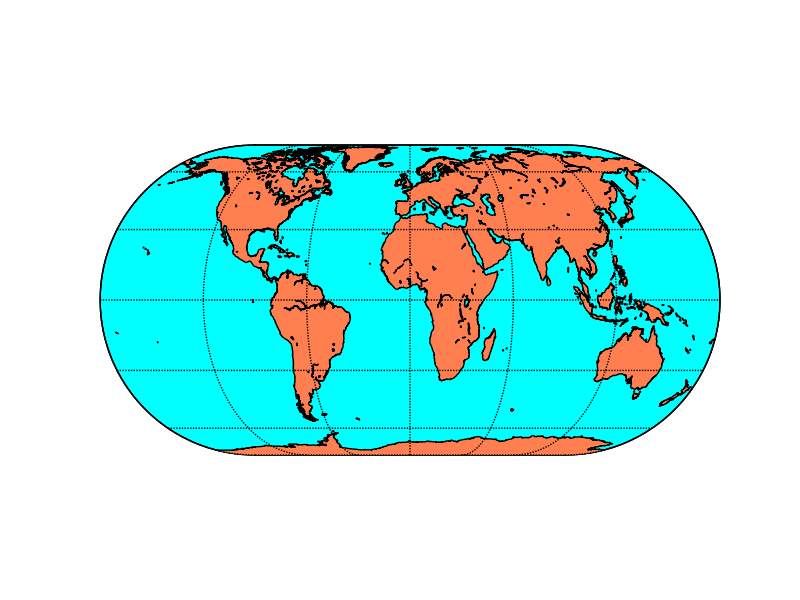
\includegraphics[scale=0.5,origin=c]{/Users/student/seminar/Kartendarstellungen/seminar/eck4} 
\caption{Eckert 4 Projektion}
\end{figure}
\newpage 